\documentclass[a4paper,10pt]{article}
\usepackage[utf8]{inputenc}
\usepackage{listings}
\usepackage{graphicx}

\lstdefinestyle{mystyle}{
    numberstyle=\tiny,
    basicstyle=\footnotesize,
    breakatwhitespace=false,         
    breaklines=true,                 
    captionpos=b,                    
    keepspaces=true,                 
    numbers=left,                    
    numbersep=5pt,                  
    showspaces=false,                
    showstringspaces=false,
    showtabs=false,                  
    tabsize=2
}
 
\lstset{style=mystyle}
 

\title{NUR Hand-in excercise 1}
\author{Meng Yao (s2308266)}

\begin{document}

\maketitle

\begin{abstract}
 The source code and the outputs of Hand-in exercise 1 are shown in this report.
\end{abstract}

\section{Source code}
\lstinputlisting{main.py}

\section{Outputs}
\lstinputlisting{outputs.txt}
\begin{figure}
    \centering
    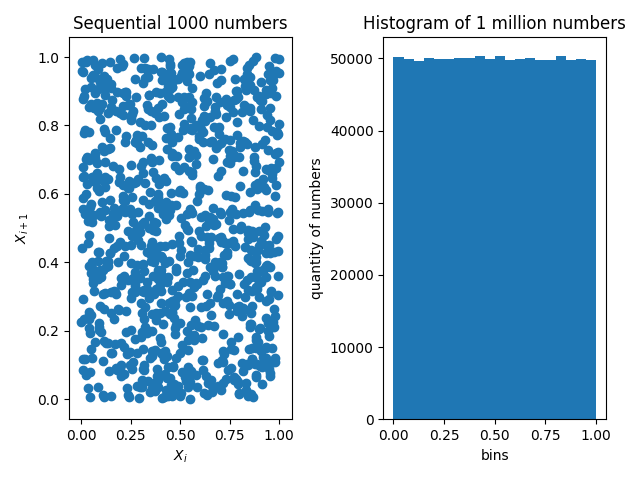
\includegraphics[width=1.\linewidth]{1.png}
    \caption{random number generator}
    \label{fig:my_label}
\end{figure}
\begin{figure}
    \centering
    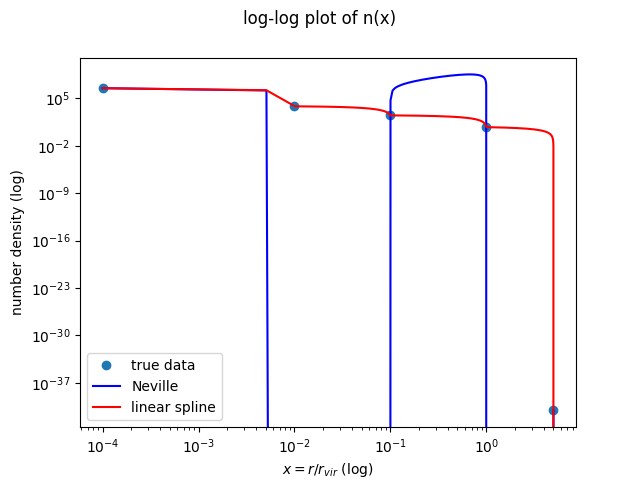
\includegraphics[width=1.\linewidth]{2b.png}
    \caption{number density and interpolations}
    \label{fig:my_label}
\end{figure}
\begin{figure}
    \centering
    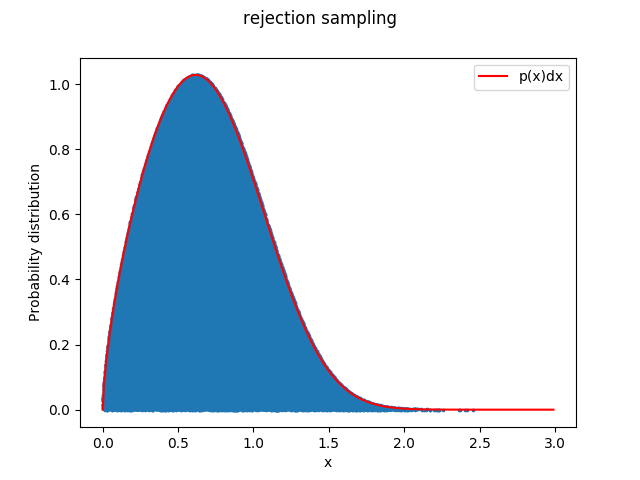
\includegraphics[width=1.\linewidth]{2d.png}
    \caption{probability distribution}
    \label{fig:my_label}
\end{figure}
\begin{figure}
    \centering
    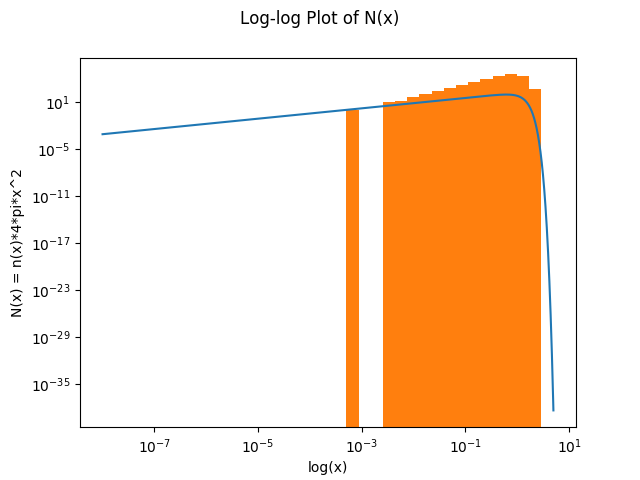
\includegraphics[width=1.\linewidth]{2e.png}
    \caption{1000 haloes and number of satellites in each bin}
    \label{fig:my_label}
\end{figure}
\begin{figure}
    \centering
    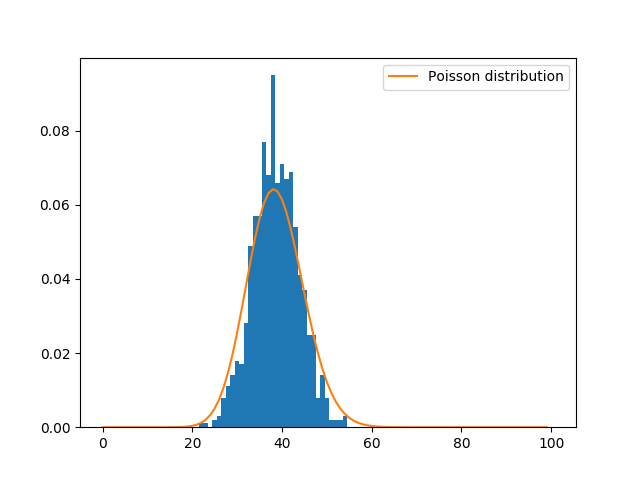
\includegraphics[width=1.\linewidth]{2g.png}
    \caption{Poisson distribution}
    \label{fig:my_label}
\end{figure}
\end{document}
